\documentclass[10pt,landscape]{article}
\usepackage{multicol}
\usepackage{calc}
\usepackage[landscape]{geometry}
\usepackage{amsmath,amsthm,amsfonts,amssymb}
\usepackage{color,graphicx,overpic}
\graphicspath{ {images/} }
\usepackage{hyperref}
\usepackage{esint}
\usepackage{bm}
\usepackage{relsize}
\usepackage{datetime}
\usepackage[utf8] {inputenc}
\usepackage[spanish, activeacute] {babel}
\usepackage{IEEEtrantools}
\usepackage{framed}

\usepackage{draftwatermark}
\SetWatermarkText{Javier de Martí­n}
\SetWatermarkScale{4.8}

% This sets page margins to .5 inch if using letter paper, and to 1cm
% if using A4 paper. (This probably isn't strictly necessary.)
% If using another size paper, use default 1cm margins.
\ifthenelse{\lengthtest { \paperwidth = 11in}}
    { \geometry{top=.5in,left=.5in,right=.5in,bottom=.5in} }
    {\ifthenelse{ \lengthtest{ \paperwidth = 297mm}}
        {\geometry{top=1cm,left=1cm,right=1cm,bottom=1cm} }
        {\geometry{top=1cm,left=1cm,right=1cm,bottom=1cm} }
    }

% Turn off header and footer
\pagestyle{empty}

% Redefine section commands to use less space
\makeatletter
\renewcommand{\section}{\@startsection{section}{1}{0mm}%
                                {-1ex plus -.5ex minus -.2ex}%
                                {0.5ex plus .2ex}%x
                                {\normalfont\large\bfseries}}
\renewcommand{\subsection}{\@startsection{subsection}{2}{0mm}%
                                {-1explus -.5ex minus -.2ex}%
                                {0.5ex plus .2ex}%
                                {\normalfont\normalsize\bfseries}}
\renewcommand{\subsubsection}{\@startsection{subsubsection}{3}{0mm}%
                                {-1ex plus -.5ex minus -.2ex}%
                                {1ex plus .2ex}%
                                {\normalfont\small\bfseries}}
\makeatother

\newcommand{\Lagr}{\mathcal{L}}

% Define BibTeX command
\def\BibTeX{{\rm B\kern-.05em{\sc i\kern-.025em b}\kern-.08em
    T\kern-.1667em\lower.7ex\hbox{E}\kern-.125emX}}

% Don't print section numbers
\setcounter{secnumdepth}{0}


\setlength{\parindent}{0pt}
\setlength{\parskip}{0pt plus 0.5ex}

%My Environments
\newtheorem{example}[section]{Example}
% ---------------------------------------------------------------

\begin{document}
\raggedright
\footnotesize
\begin{multicols}{3}


% multicol parameters
% These lengths are set only within the two main columns
%\setlength{\columnseprule}{0.25pt}
\setlength{\premulticols}{1pt}
\setlength{\postmulticols}{1pt}
\setlength{\multicolsep}{1pt}
\setlength{\columnsep}{2pt}

\begin{framed}
	\begin{center}
    	\Large{\underline{Campos Electromagnéticos}} \\
    	\scriptsize{2º Curso de Ingeniería de Telecomunicaciones | UPV/EHU}\\
     	%Actualizado por última vez el \today \\
     	"\textsl{Under-promise and over-deliver}." \\
     	%\hspace{5 pt} \\
     	\small{\textbf{Javier de Martín Gil -- 2015/16}}
	\end{center}
\end{framed}

\section{\underline{Introducción y Ondas Planas}}

\textbf{Longitud de onda} en un medio:

\begin{equation*}
	\lambda = \frac{v}{f} = \frac{c}{f \cdot n} = \frac{c}{f \cdot \sqrt{{\mu_{r_x}} \epsilon_{r_x}}} 
\end{equation*}

\textbf{Impedancia intrínseca} de un medio:

\begin{equation*}
	Z_x = \sqrt{\frac{\mu_x}{\epsilon_x}} = \sqrt{\frac{\mu_{r_x} \cdot \mu_0}{\epsilon_{r_x} \cdot \epsilon_0}}		
\end{equation*}

Una onda plana tiene la siguiente expresión:

\begin{equation*}
	\vec{E}(x, y, z) = \vec{E_0} e^{-j \beta \hat{u}}
\end{equation*}

Se cumple la \textbf{condición de perpendicularidad} entre el campo magnético y la dirección de propagación: $\vec{E_0} \cdot \beta \hat{u} = 0$ \\

\textbf{Polarización} de ondas planas:

\begin{itemize}
    \item \textbf{Lineal}: $\mathbb{R}[E_0] \parallel \mathbb{I}[E_0]$
    \item \textbf{Circular}: $\mathbb{R}[E_0] \perp \mathbb{I}[E_0]$ y $| \mathbb{R}[E_0]| = | \mathbb{I}[E_0]|$
    \item \textbf{Elíptica}: En el resto de los casos
\end{itemize}

El \textbf{sentido de giro} para polarización elíptica o circular:

\begin{equation*}
    \vec{u} \cdot (\mathbb{R}[E_0] \times \mathbb{I}[E_0]) = \begin{cases}
                                                                > 0 \mbox{ Negativa/Anti-horario/Levógiro} \\
                                                                < 0 \mbox{ Positiva/Horario/Dextrógiro}
                                                        \end{cases}
\end{equation*}

%     ____           _     __                _          _   __                           __
%    /  _/___  _____(_)___/ /__  ____  _____(_)___ _   / | / /___  _________ ___  ____ _/ /
%    / // __ \/ ___/ / __  / _ \/ __ \/ ___/ / __ `/  /  |/ / __ \/ ___/ __ `__ \/ __ `/ / 
%  _/ // / / / /__/ / /_/ /  __/ / / / /__/ / /_/ /  / /|  / /_/ / /  / / / / / / /_/ / /  
% /___/_/ /_/\___/_/\____/\___/_/ /_/\___/_/\__,_/  /_/ |_/\____/_/  /_/ /_/ /_/\__,_/_/   
                                                                                         
\section{\underline{Incidencia Normal}}

\subsection{Incidencia Normal en dos medios}

%\begin{center}
%	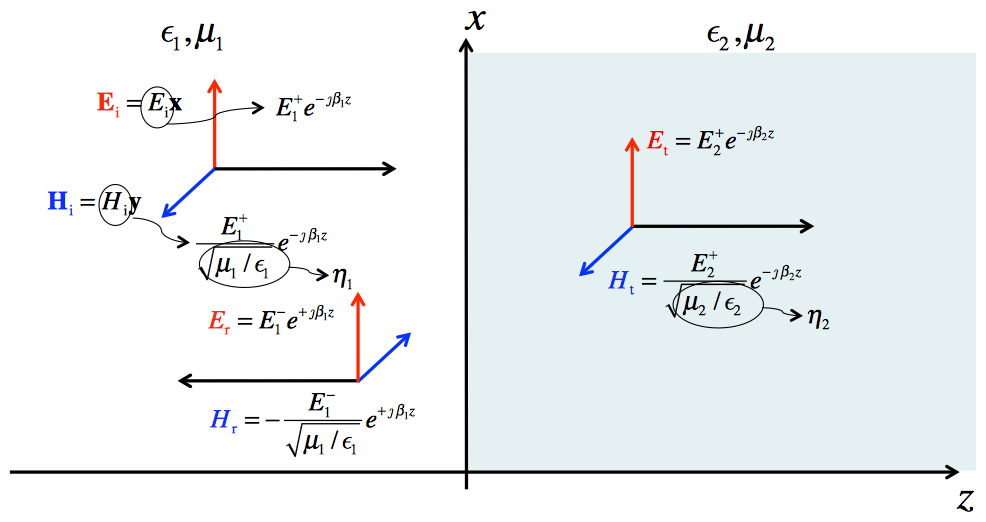
\includegraphics[scale = 0.18]{images/Incidencia_Normal_2Medios}
%\end{center}

\begin{equation*}
	E_1^+ + E_1^- = E_2^+
\end{equation*}

\textbf{Coeficiente de reflexión} ($\rho$): \\

\begin{equation*}
	\rho = \frac{\eta_2 - \eta_1}{\eta_2 + \eta_1}
\end{equation*}

\textbf{Coeficiente de transmisión} ($\tau = 1 + \rho$): \\

\begin{equation*}
	\tau = \frac{2 \eta_2}{\eta_2 + \eta_1}
\end{equation*}

\textbf{Porcentaje de potencia reflejada}:

\begin{equation*}
	P_{\%} = |\rho|^2 \cdot 100\%
\end{equation*}

\textbf{Potencia}:

\begin{equation*}
    P = \frac{|\vec{E}_0|^2}{2 \eta}
\end{equation*}

Se puede establecer una relación entre la potencia transmitida y la recibida:

\begin{equation*}
	\frac{P_t}{P_r} = e^{-2\alpha z}
\end{equation*}

\textbf{Pérdidas} de un medio: $tan(\delta) = x$. La \textbf{atenuación} de un medio con pérdidas es:

\begin{equation*}
	\alpha = \beta \frac{\tan (\delta)}{2}
\end{equation*}


Una onda que incide en una discontinuidad se descompone en tres:

\begin{itemize}
    \item \textbf{Onda Incidente}: \\
        \quad{$\vec{E_i} = E_1^+ e^{-j\beta_1 z}$}
        \quad{$\vec{H_i} = \frac{H_1^+}{\sqrt{ \mu_1 / \epsilon_1}} e^{-j\beta_1 z}$}
    \item \textbf{Onda Reflejada}:\\
        \quad{$\vec{E_r} = E_1^- e^{+j\beta_1 z}$}
        \quad{$\vec{H_r} = \frac{H_1^+}{\sqrt{ \mu_1 / \epsilon_1}} e^{+j\beta_1 z}$}
    \item \textbf{Onda Transmitida}: \\
        \quad{$\vec{E_t} = E_2^+ e^{-j\beta_1 z}$}
        \quad{$\vec{H_t} = \frac{H_2^+}{\sqrt{ \mu_2 / \epsilon_2}} e^{-j\beta_1 z}$}
\end{itemize}

\textbf{Coeficiente de onda estacionaria (\textit{COE})}: Relaciona la cantidad de energía emitida por el emisor y la cantidad de energía reflejada de vuelta.\\

\begin{equation*}
	s = \frac{1 + |\rho|}{1 - |\rho|}
\end{equation*}
    
\subsection{Incidencia normal en tres medios}

%La impedancia del tercer medio semi-infinito, es igual la impedancia que ve la onda desde la superficie $z = D$. \\

\begin{equation*}
	\rho_{23} = \frac{Z_{23} - \eta_2}{Z_{23} + \eta_2} = \frac{\eta_3 - \eta_2}{\eta_3 + \eta_2} \hspace{10 pt} \rho_{12} = \frac{Z_{12} - \eta_1}{Z_{12} - \eta_1}
\end{equation*}

\begin{equation*}
	Z_{12} = \eta_2 \frac{Z_{23} \cdot cos(\beta_2 d_2) + \eta_2 \cdot j sin(\beta_2 d_2)}{\eta_2 \cdot cos(\beta_2 d_2) + Z_{23} \cdot j sin(\beta_2 d_2)} \hspace{15 pt} Z_{23} = \eta_3
\end{equation*}



\subsection{Supresión de reflexiones en el primer medio}

($A$ y $B$ son los medios de las caras externas y $X$ el medio intermedio)

\begin{equation*}
	\beta_x = \beta_0 \cdot n_x
\end{equation*}

\textbf{Ventana Dieléctrica}

\begin{equation*}
	sin(\beta_x D_x) = 0 \hspace{5 pt} \begin{cases}
  							\eta_b = \eta_a \\
  							D_x = n \frac{\lambda_x}{2} \hspace{5 pt} n = 1, 2,...
						\end{cases}
\end{equation*}

\textbf{Transformador de Lambda Cuartos}

\begin{equation*}
	cos(\beta_x D_x) = 0 \hspace{5 pt} \begin{cases}
  							\eta_x = \sqrt{\eta_a \eta_b} \\
  							D_x = (2n - 1) \frac{\lambda_x}{4} \hspace{5 pt} n = 1, 2,...
						\end{cases}
\end{equation*}

\subsection{Incidencia Normal en Medios con N Discontinuidades}

Comenzar los cálculos desde el último medio, de atrás hacia delante, como en el caso de 3 medios.

%     ____           _     __                _          ____  __    ___                 
%    /  _/___  _____(_)___/ /__  ____  _____(_)___ _   / __ \/ /_  / (_)______  _______
%    / // __ \/ ___/ / __  / _ \/ __ \/ ___/ / __ `/  / / / / __ \/ / / ___/ / / / __ `/
%  _/ // / / / /__/ / /_/ /  __/ / / / /__/ / /_/ /  / /_/ / /_/ / / / /__/ /_/ / /_/ / 
% /___/_/ /_/\___/_/\__,_/\___/_/ /_/\___/_/\__,_/   \____/_.___/_/_/\___/\__,_/\__,_/  
                                                                                      
\section{\underline{Incidencia Oblicua}}

%\begin{center}
%	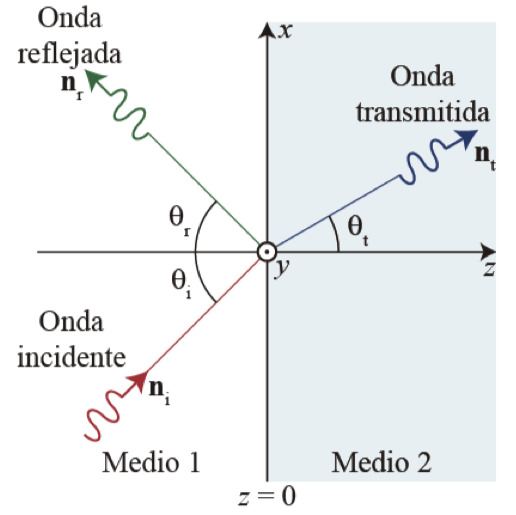
\includegraphics[scale = 0.15]{images/Incidencia_Oblicua}
%\end{center}

\begin{itemize}
	\item $\theta_i$ es el ángulo de incidencia, $\theta_r$ es el ángulo de reflexión y $\theta_t$ es el ángulo de transmisión/refracción.
	\item Plano de incidencia es el plano que contiene el vector normal a la superficie ($z$) y $\hat{n}_e$, $\hat{n}_i$ y $\hat{n}_t$. \\
\end{itemize}

%\subsection{Leyes de Snell. Índice de Refracción. Reflexión Total}

Todas las ondas que se propaguen en un mismo medio tienen la misma velocidad de fase ($v_f$). \\

\textbf{Leyes de Snell}:

\begin{enumerate}
    \item \textbf{Ley de la Reflexión}: Las ondas incidente y reflejada están en el mismo medio ($v_{f_1} = v_{f_2}$): $\theta_r = \theta_i$
        
    \item \textbf{Ley de la Refracción}: Las ondas incidente y transmitida están en medios distintos ($v_{f_1} \neq v_{f_2}$) 
        \begin{equation*}
            sin(\theta_t) = \frac{v_{f_1}}{v_{f_2}} \cdot sin(\theta_i) \hspace{15 pt} n_2 sin(\theta_t) = n_1 sin(\theta_i)
        \end{equation*}
\end{enumerate}

El \textbf{índice de refracción} ($n_x$) compara la velocidad de fase de una \textit{OEM} propagándose en un medio determinado con la velocidad de fase $c$ que tendría en el vacío:

\begin{equation*}
	n_x = \frac{c}{v_f} = \sqrt{\mu_{rx} \epsilon_{rx}}
\end{equation*}

Dependiendo del valor del índice de refracción del medio hay que distinguir dos casos:

\begin{equation*}
	n_x < n_{x+1} \rightarrow \theta_t < \theta_i \hspace{15 pt} n_x > n_{x+1} \rightarrow \theta_t > \theta_i
\end{equation*}

A medida que aumenta el ángulo de incidencia $\theta_i$ aumenta aún más el ángulo de transmisión $\theta_t$. El límite es $\theta_t = 90º$, es el \textbf{ángulo crítico} ($\theta_c$). Por encima del ángulo crítico no existe onda transmitida, la onda incidente se refleja totalmente produciendo el fenómeno de \textbf{reflexión total}.

\begin{equation*}
    \theta_c = \arcsin \left( \frac{n_{x+1}}{n_x} \right)
\end{equation*}

\subsection{Descomposición del Campo Eléctrico Incidente en el Plano de Incidencia}

La fórmula general para escribir una onda es:

\begin{equation*}
	\vec{E}_x = \vec{E}_{xo} \cdot e^{-j \beta \hat{u}}
\end{equation*}

Para determinar las amplitudes de las ondas reflejada y transmitida, es conveniente descomponer la onda incidente respecto al plano de incidencia.

\begin{equation*}
    \vec{E_i} = \vec{E_{i_\perp}} + \vec{E_{i_\parallel}}
\end{equation*}

\subsubsection{Polarización Paralela}



Para un ángulo de incidencia determinado, ángulo de polarización $\theta_p = arctan(n_2 / n_1)$, $\rho_\parallel = 0$, no se refleja.

%\begin{center}
%	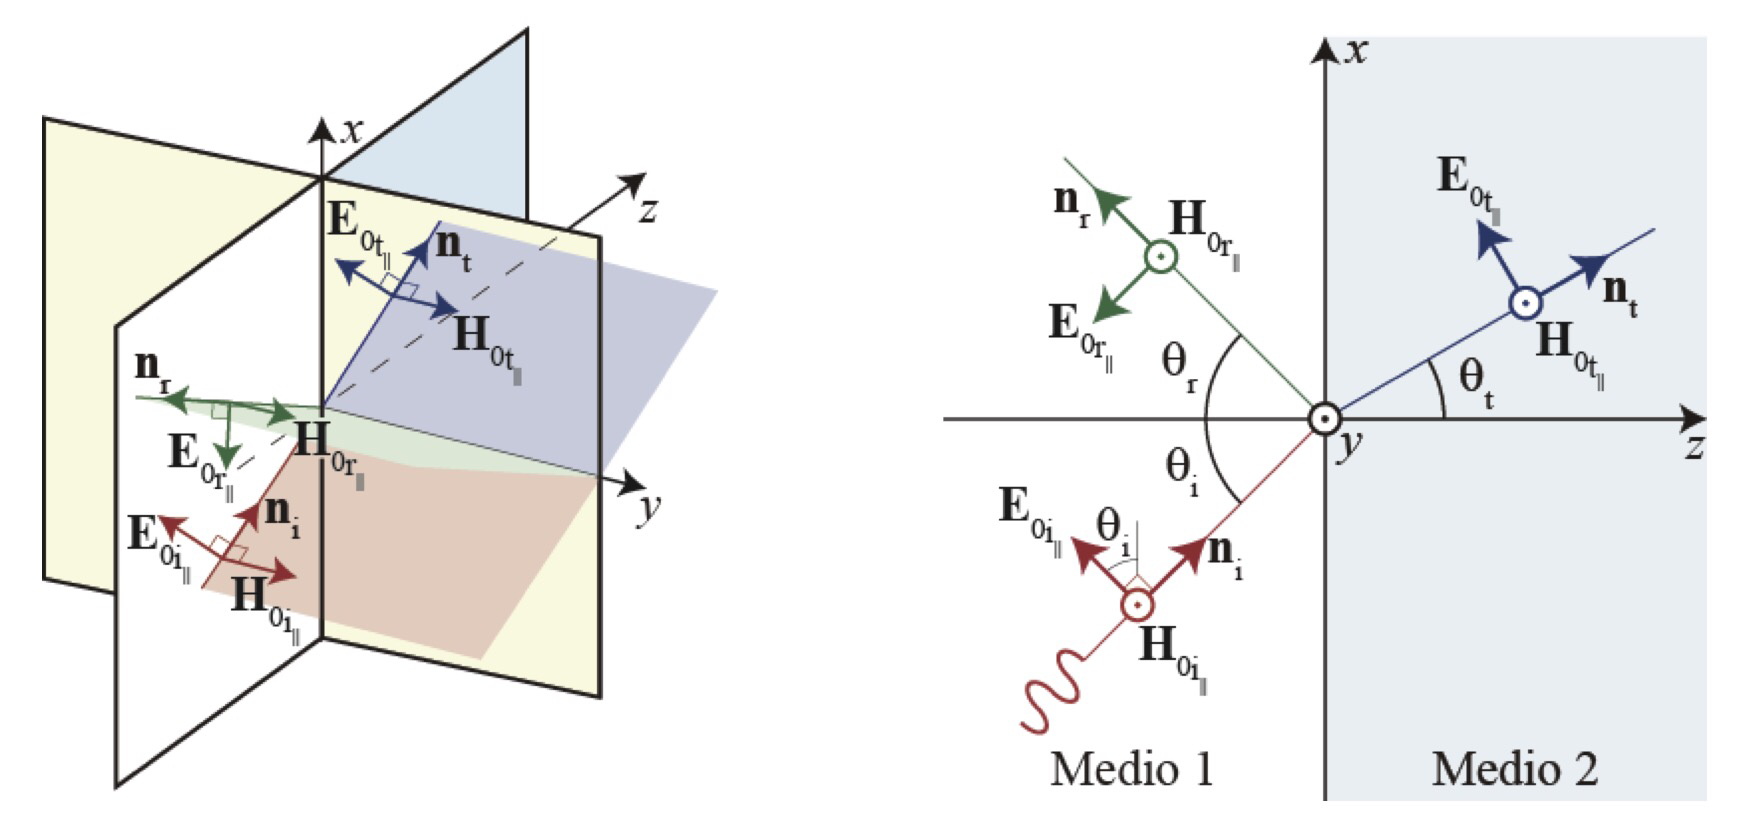
\includegraphics[scale = 0.08]{images/Polarizacion_Paralela}
%\end{center}

\begin{equation*}
	E_{0_{r_\parallel}} = \rho_\parallel \cdot E_{0_{i_\parallel}} \hspace{20 pt} E_{0_{t_\perp}} = \tau_\parallel \cdot E_{0_{i_\perp}}
\end{equation*}

\textbf{Coeficiente de reflexión}:

\begin{equation*}
    \rho_\parallel = \frac{\eta_2 cos{\theta_t} - \eta_1 cos{\theta_i}}{\eta_2 cos{\theta_t} + \eta_1 cos{\theta_i}} = \frac{ \left. E_{0_{r_{\parallel}}} \right|_{tang} }{ \left. E_{0_{i_{\parallel}}} \right|_{tang}}
\end{equation*}

\textbf{Coeficiente de transmisión}:

\begin{equation*}
    \tau_\parallel = \frac{2 \eta_2 cos{\theta_t}}{\eta_2 cos{\theta_t} + \eta_1 cos{\theta_i}} = \frac{ \left. E_{0_{t_{\parallel}}} \right|_{tang} }{ \left. E_{0_{i_{\parallel}}} \right|_{tang}}
\end{equation*}

\subsubsection{Polarización Perpendicular}

Una onda con polarización perpendicular \textbf{siempre se reflejará} ($\rho_\perp \neq 0$) independientemente del ángulo de incidencia.

%\begin{center}
%	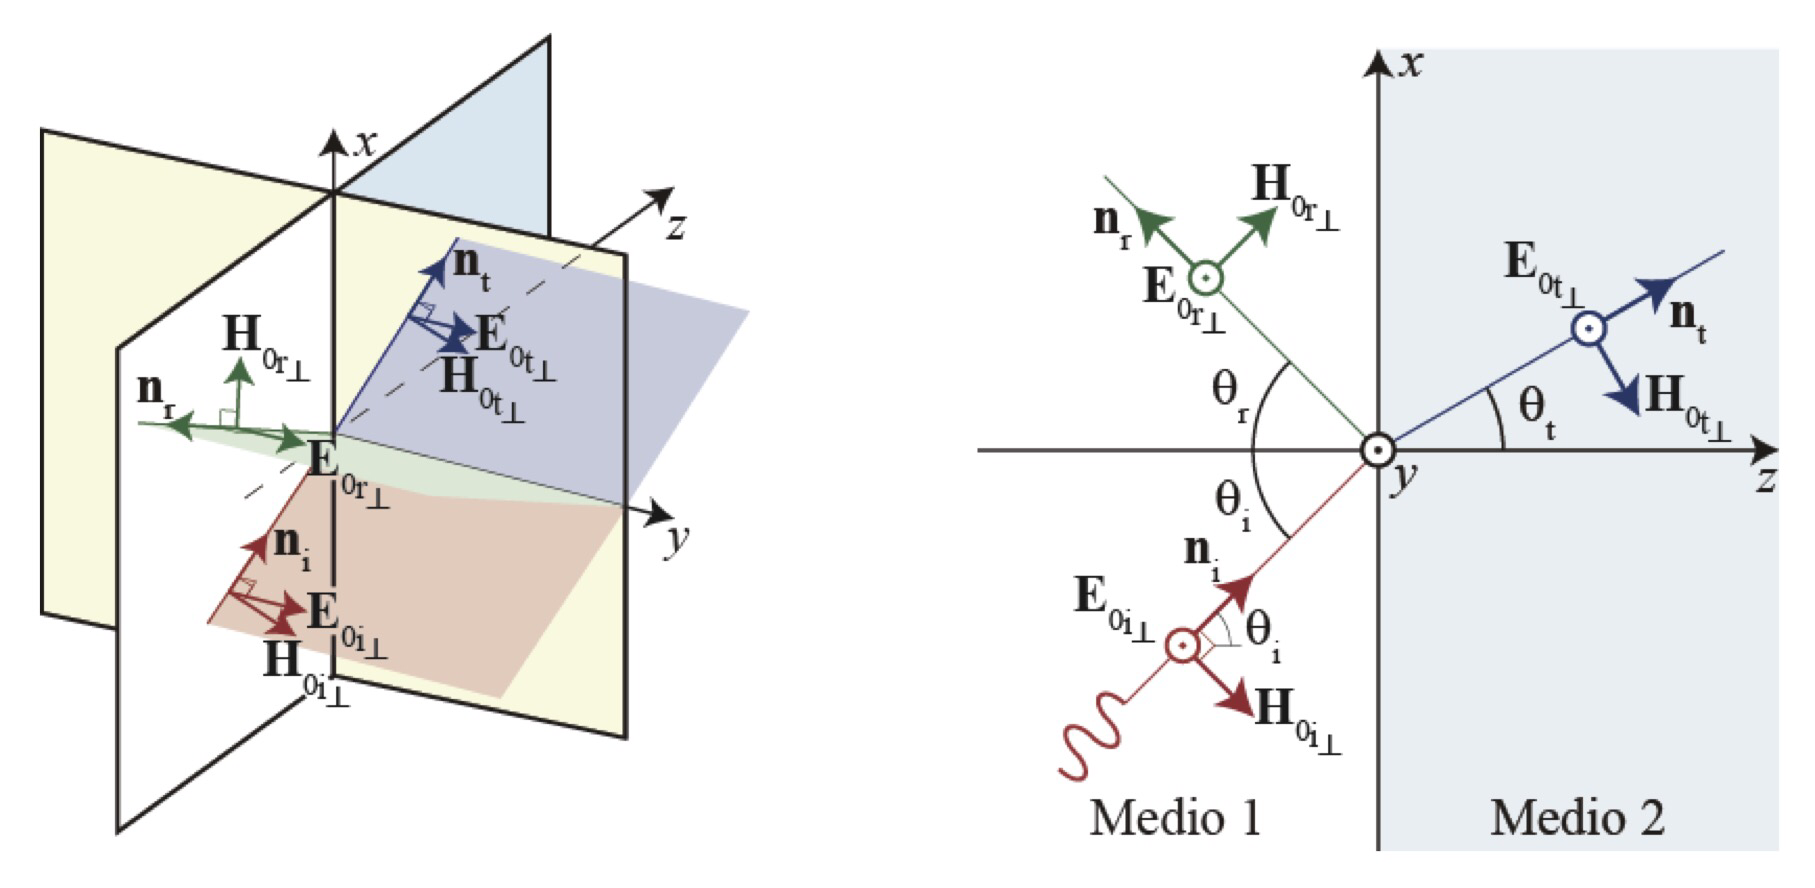
\includegraphics[scale = 0.08]{images/Polarizacion_Perpendicular}
%\end{center}

\begin{equation*}
	E_{0_{r_\perp}} = \rho_\perp \cdot E_{0_{i_\perp}} \hspace{20 pt} E_{0_{t_\perp}} = \tau_\perp \cdot E_{0_{i_\perp}} 
\end{equation*} 

\textbf{Coeficiente de reflexión}:

\begin{equation*}
    \rho_\perp = \frac{\eta_2 sec{\theta_t} - \eta_1 sec{\theta_i}}{\eta_2 sec{\theta_t} + \eta_1 sec{\theta_i}} = \frac{ \left. E_{0_{r_{\perp}}} \right|_{tang} }{ \left. E_{0_{i_{\perp}}} \right|_{tang}}
\end{equation*}

\textbf{Coeficiente de transmisión}:

\begin{equation*}
    \tau_\parallel = \frac{2 \eta_2 sec{\theta_t}}{\eta_2 sec{\theta_t} + \eta_1 sec{\theta_i}} = \frac{ \left. E_{0_{t_{\perp}}} \right|_{tang} }{ \left. E_{0_{i_{\perp}}} \right|_{tang}}
\end{equation*}

La \textbf{dirección del campo magnético}, para ambos casos de polarización, se puede conseguir:

\begin{equation*}
	\vec{H} = \frac{\hat{n} \wedge \vec{E_0}}{\eta}
\end{equation*}

Observaciones sobre los coeficientes de reflexión en las polarizaciones perpendicular y paralela.

\begin{itemize}
	\item $|\rho_\perp| > |\rho_\parallel|$
	\item $\rho_\perp \neq \rho_\parallel$
	\item Si la \textbf{incidencia es oblicua no se mantiene la polarización}.
\end{itemize}

%    ______      __                  __        ____            __     
%   / ____/_  __/_/___ ______   ____/ /__     / __ \____  ____/ /_____
%  / / __/ / / / / __ `/ ___/  / __  / _ \   / / / / __ \/ __  / __  /
% / /_/ / /_/ / / /_/ (__  )  / /_/ /  __/  / /_/ / / / / /_/ / /_/ / 
% \____/\__,_/_/\__,_/____/   \__,_/\___/   \____/_/ /_/\__,_/\__,_/  
                                                                    

\section{\underline{Guías de Onda}}

Se establecen las siguientes condiciones de contorno: $E_y(x = 0) = E_y(x = a) = 0$.

\begin{equation*}
	\vec{\beta} = \beta_x \hat{x} + \beta_y \hat{y} + \beta_z \hat{z} \mbox{ ,}\quad \lambda = \frac{2\pi}{\beta}
\end{equation*}

\begin{itemize}
    \item \textbf{Velocidad de fase}: es la tasa a la cual la fase de la misma se propaga en el espacio.
    	\begin{equation*}
    		v_{f} = \frac{L_z}{\lambda} c = \frac{\beta}{\beta_z}	c = \frac{\omega}{\beta_z} = \frac{c}{\sqrt{\epsilon_r} \sqrt{1 - \left( \frac{\omega_c}{\omega}\right) ^2}} > c
    	\end{equation*}

    \item \textbf{Velocidad de grupo}: velocidad a con la que las variaciones en la forma de la amplitud de la onda se propagan en el espacio.
    	\begin{equation*}
    		v_{g} = v_{prop} = \frac{\partial \omega}{\partial \beta_z} = \frac{\beta_z}{\beta}c = \frac{\omega}{\beta_z} = \frac{c}{\sqrt{\epsilon_r}} \sqrt{1 - \left( \frac{\omega_c}{\omega}\right) ^2} < c	
    	\end{equation*}
\end{itemize}

La \textbf{ecuación de onda} es:

\begin{equation*}
	E(x, y, z) = E_0 \cdot {\overbrace{cos(\omega t - \beta_z z)}^{\text{Onda viajera}}}
                         {\underbrace{sin(\beta_x x)	}}_{\text{Onda estacionaria}}	
\end{equation*}

\begin{equation*}
	\omega^2 = (\beta_x^2 + \beta_z^2) c^2
\end{equation*}


\textbf{Relación de dispersión}, relaciona la longitud de onda o el número de onda con su frecuencia:

\begin{equation*}
    \omega = c \sqrt{ \left( \frac{n \pi}{a} \right) ^2 + \beta^2_z}
\end{equation*}

\begin{equation*}
	- \gamma_c^2 \triangleq \omega^2 \mu \epsilon + \gamma^2 = \omega_c^2 \mu = \frac{\omega_c^2}{c}
\end{equation*}

\textbf{Atenuación}:

\begin{equation*}
	\alpha (dB) = \frac{2 \pi}{c} \sqrt{f_{dominante}^2 - f_t^2}
\end{equation*}

\begin{equation*}
	\alpha (Np/m) = \frac{\alpha (dB/m)}{20 \cdot log_{10}(e)}
\end{equation*}

\textbf{Longitud de Onda de la Guía de Ondas}:

\begin{equation*}
	\lambda_g = \frac{v_{fase}}{f} = \frac{\lambda}{ \sqrt{1 - \left( \frac{\omega_c}{\omega}\right) ^2}}
\end{equation*}


\subsection{Modos de Propagación}

\begin{itemize}
	\item \textbf{Modo Transversal Electro-Magnético} ($E_z = H_z = 0$): No existe ninguna componente del campo eléctrico en la dirección de propagación.
	\item \textbf{Modo Transversal Magnético} ($H_z = 0$): No existe ninguna componente del campo magnético en la dirección de propagación.
	\item \textbf{Modo Transversal Eléctrico} ($E_z = 0$): No existe ninguna componente del campo eléctrico en la dirección de propagación.
\end{itemize}

\textbf{Frecuencia de corte} de un modo $mn$ de propagación:

\begin{equation*}
	f_{c_{mn}} = \frac{c}{2 \pi \sqrt{\epsilon_r}} \sqrt{ \left( \frac{m \pi}{a} \right)^2 + \left( \frac{n \pi}{b} \right)^2 }
\end{equation*}

El \textbf{ancho de banda} de una guía de ondas es la diferencia entre el modo fundamental y el primer modo superior.\\

El \textbf{desfase de la onda} al atravesar la guía se puede expresar como: $\phi = L \cdot \beta$

\textbf{Retardo de propagación} que sufre la onda al atravesar la guía: $\gamma = \frac{L}{v_{g}} (segundos)$

El \textbf{modo dominante} de una guía de ondas es aquel con la frecuencia más baja.


%     __    _                              __        _______  __
%    / /   (_)___  ___  ____ ______   ____/ /__     /_  __/ |/ /
%   / /   / / __ \/ _ \/ __ `/ ___/  / __  / _ \     / /  |   / 
%  / /___/ / / / /  __/ /_/ (__  )  / /_/ /  __/    / /  /   |  
% /_____/_/_/ /_/\___/\__,_/____/   \__,_/\___/    /_/  /_/|_|  
                                                              

\section{\underline{Líneas de Transmisión}}

\begin{center}
	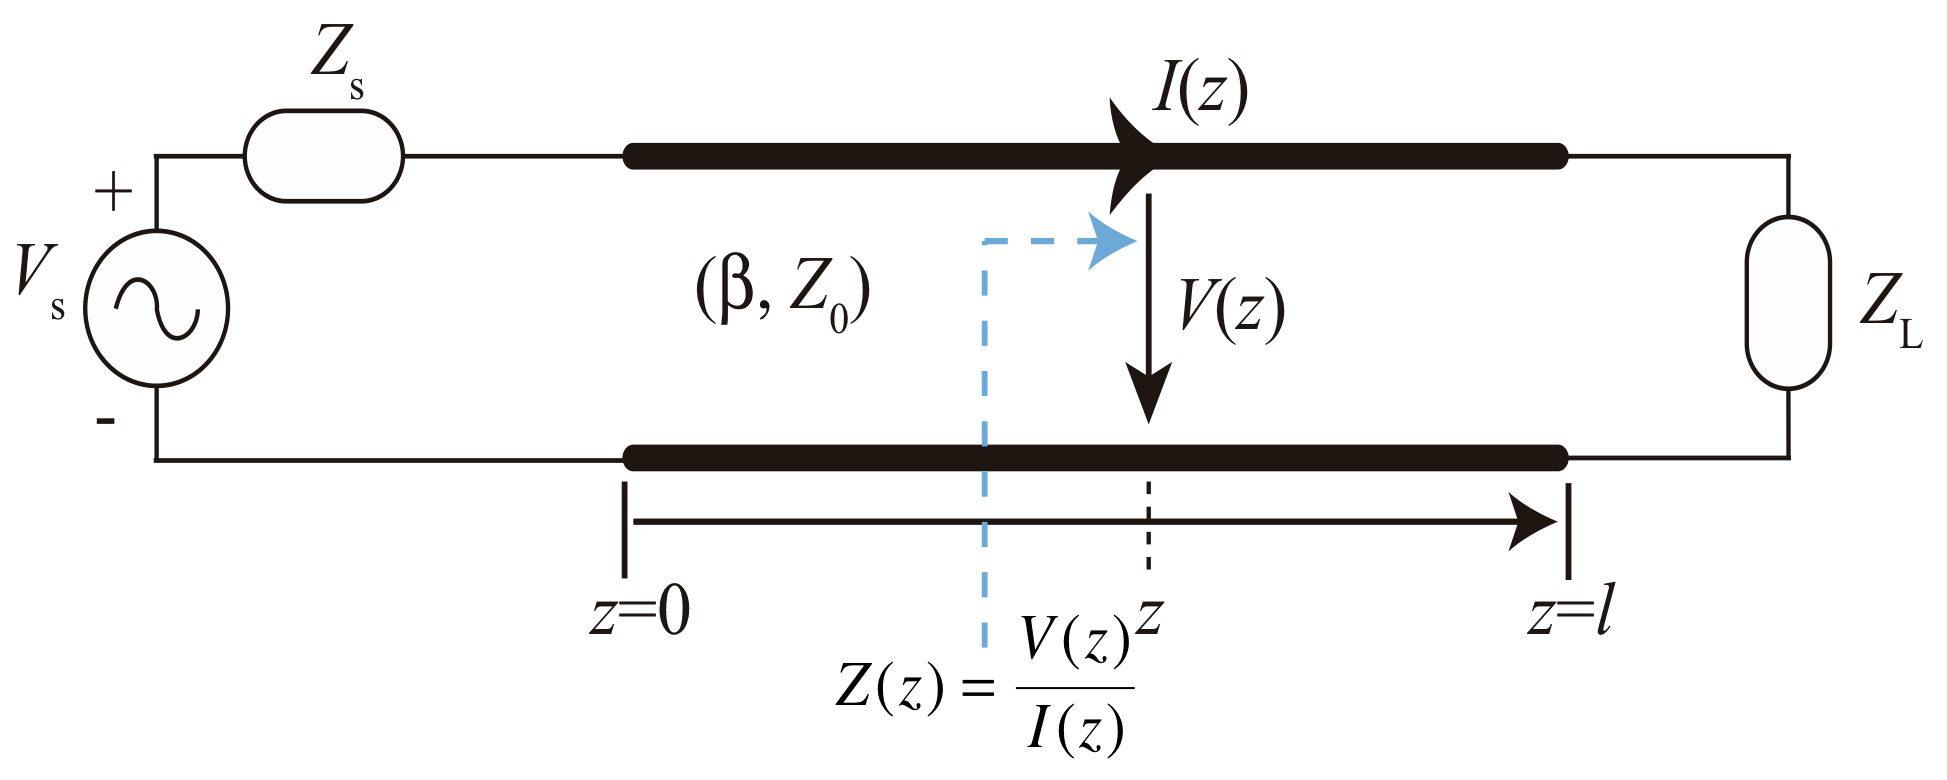
\includegraphics[scale = 0.08]{images/Linea_TX.png}
\end{center}

\textbf{Coeficiente de reflexión} en la carga ($z$): 

\begin{equation*}
	\rho = \frac{V_0^- \cdot e^{+ j \beta z}}{V_0^+ \cdot e^{-j \beta z}} = \frac{Z_L - Z_0}{Z_L + Z_0}
\end{equation*}

\textbf{Coeficiente de reflexión} en una posición arbitraria:

\begin{equation*}
	\rho(l) = \rho_L \cdot e^{-2 \gamma l}
\end{equation*}

\textbf{Impedancia}:

\begin{equation*}
	Z(0) = Z_0 \frac{Z(l) cos(\beta l) + j Z(0) sin(\beta l)}{Z(0) cos(\beta l) + j Z(l) sin(\beta l)}
\end{equation*}

\textbf{Impedancia de entrada} en $Z(z)$:

\begin{equation*}
	Z(z) = \frac{V(z)}{I(z)} = Z_0 \frac{1 + \rho(z)}{1 - \rho(z)}
\end{equation*}

\begin{equation*}
	\rho(z) = \rho(0) e^{2 j \beta z} \hspace{5 pt} \rho(l) = \rho_l \frac{Z_l - Z_0}{Z_l + Z_0}
\end{equation*}

\textbf{Coeficiente de Onda Estacionaria}:

\begin{equation*}
	s = \frac{|V_{max}|}{|V_{min}|} = \frac{1 + |\rho|}{1 - |\rho|}
\end{equation*}

\textbf{Tensión en un punto de la guía}:

\begin{equation*}
	V(z) = V_0^+ e^{-j \beta z} + V_0^- e^{j \beta z}
\end{equation*}

\textbf{Corriente en un punto de la guía}:

\begin{equation*}
	I(z) = \frac{V_0^+}{Z_0} e^{-j \beta z} + \frac{V_0^-}{Z_0} e^{j \beta z}	
\end{equation*}

\subsection{Transformación de Impedancias}

\begin{itemize}
	\item \textbf{Cortocircuito}: $Z_L = 0$, $\rho_L = -1$
	\item \textbf{Circuito Abierto}: $Z_L \rightarrow \infty$, $\rho_L = +1$
	\item \textbf{Línea de Transmisión y Carga Adaptadas}: $Z_L = Z_0$, $\rho_L = 0$
	\item \textbf{Línea de Transmisión y Fuente Adaptadas}: $Z(0) = Z_S$
\end{itemize}

\textbf{Coeficiente de Onda Estacionaria (\textit{COE})}:

\begin{equation*}
	s = \frac{V_{max}}{V_{min}} = \frac{1 + |\rho(z)|}{1 - |\rho(z)|}
\end{equation*}

Valor de tensión de la onda incidente/reflejada:

\begin{equation*}
	V_0^{\pm} = \frac{1}{2} (V_0 \pm I_0 Z_0)
\end{equation*}

\textbf{Distancia al primer mínimo} ($Z_{min}$): $\phi -2 \beta Z_{min} = - \pi$

\textbf{Distancia al primer máximo} ($Z_{max}$): $\phi - 2 \beta Z_{max} = 0$


\textbf{Potencia en la carga}:

\begin{equation*}
	P_L = \frac{1}{2} \left| \frac{V_S}{Z_S + Z(0)} \right|^2 \mathbb{R}(Z_L)
\end{equation*}

\textbf{Módulo de tensión total} dentro de la línea de transmisión:

\begin{equation*}
	|V(z')| = |V_L^+| \sqrt{1 + |\rho_L|^2 + 2 |\rho| cos(\theta_L - 2 \beta z')}
\end{equation*}

%\vfill


\end{multicols}
\end{document}